%%%%%%%%%%%%%%%%%%%
%% KAPITEL Intro %%
%%%%%%%%%%%%%%%%%%%
\section{Einführung}
% MARCO
% was ist es, wer benutzt es, wofür braucht man es
% erreichbar durch Transaktion SWDD, im SAP System eingebaut usw
%%%%%%%%%%%%%%%%%%%%%%%%%%%%%%%%%%%%%%%%%%%%%%%%%%%%%%%%%%%%%%%%%
% http://www.connexin.net/de/sap-transaktionen-uebersicht.html
% -> Hier auch die Workflow transaktionen mit LOG etc erwähnen!
% http://help.sap.com/saphelp_nw04s/helpdata/EN/c5/e4b79d453d11d189430000e829fbbd/content.htm
% -> Bild zum Beispiel für die Übersicht des Builders zu erklären
% http://www.sdn.sap.com/irj/scn/go/portal/prtroot/docs/library/uuid/3c2b9c90-0201-0010-ab86-a574c7881607?QuickLink=index&overridelayout=true&5003637211723
% -> schöne Definitionen und Übersicht des Builders
% http://www.edv-buchversand.de/sap/chapter.php?cnt=getchapter&id=gp-9285.pdf
% -> auch sehr gut für Übersicht!!
% http://www.abap-tutorials.com/wp-content/uploads/pdfs/workflow_tutorial.pdf
% -> geil für die Einführung mit Warum brauchen wir überhaupt Workflows etc..
\subsection{Warum ein SAP Workflow Builder?}
\label{sec:warum-wf-builder}
Durch eine sehr breite Produktpalette und lange Erfahrung ist in einem \gls{sap} System standardmäßig eine sehr große Menge an Arbeitsabläufen vorhanden und direkt einsetzbar. Aufgrund der Verschiedenheit individueller Firmen und Branchen ist es allerdings unmöglich, alle möglichen Workflows zu integrieren und zur Verfügung zu stellen. Daher stellt die \gls{sap} ihren Kunden eine Möglichkeit zur Verfügung, mit der sie, nach einer gewissen Einarbeitungszeit, beliebige Workflows selbst abbilden können. Dadurch können gekaufte Produkte mit einer maximalen Genauigkeit in die vorhandenen Betriebsabläufe zu integriert und auch schon vorhandene Fremdsysteme angesprochen werden \cite{SAPHelpWf}.

\subsubsection{Vorteile des SAP Workflow Builders}
\label{sec:vorteile-sap-wf-builder}
Durch die direkte Einbindung in das \gls{sap} System hat der Workflow Builder einige Möglichkeiten und Funktionen, die mit einem externen Programm nicht umsetzbar wären. So ist es möglich, auf interne Ereignisse zu warten und auf diese zu reagieren. Des weiteren können auch globale Ereignisse ausgelöst werden und es kann problemlos mit anderen Transaktionen des Systems zusammengearbeitet werden. 

Da viele Firmen zur Verwaltung der Produktion, des Personals und anderen Dingen größtenteils \gls{sap} Systeme im Einsatz haben, ist es somit möglich, ein Maximum an Automatisierung zu erreichen.

\subsection{Programmoberfläche}
\label{sec:win-overwiev}
Die Programmoberfläche des Workflow Builders (siehe \ref{abb:workflow-overview}) ist in verschiedene Bereiche unterteilt. Die wichtigsten sind die im Folgenden beschriebenen.

\begin{figure}[h]
	\begin{center}
	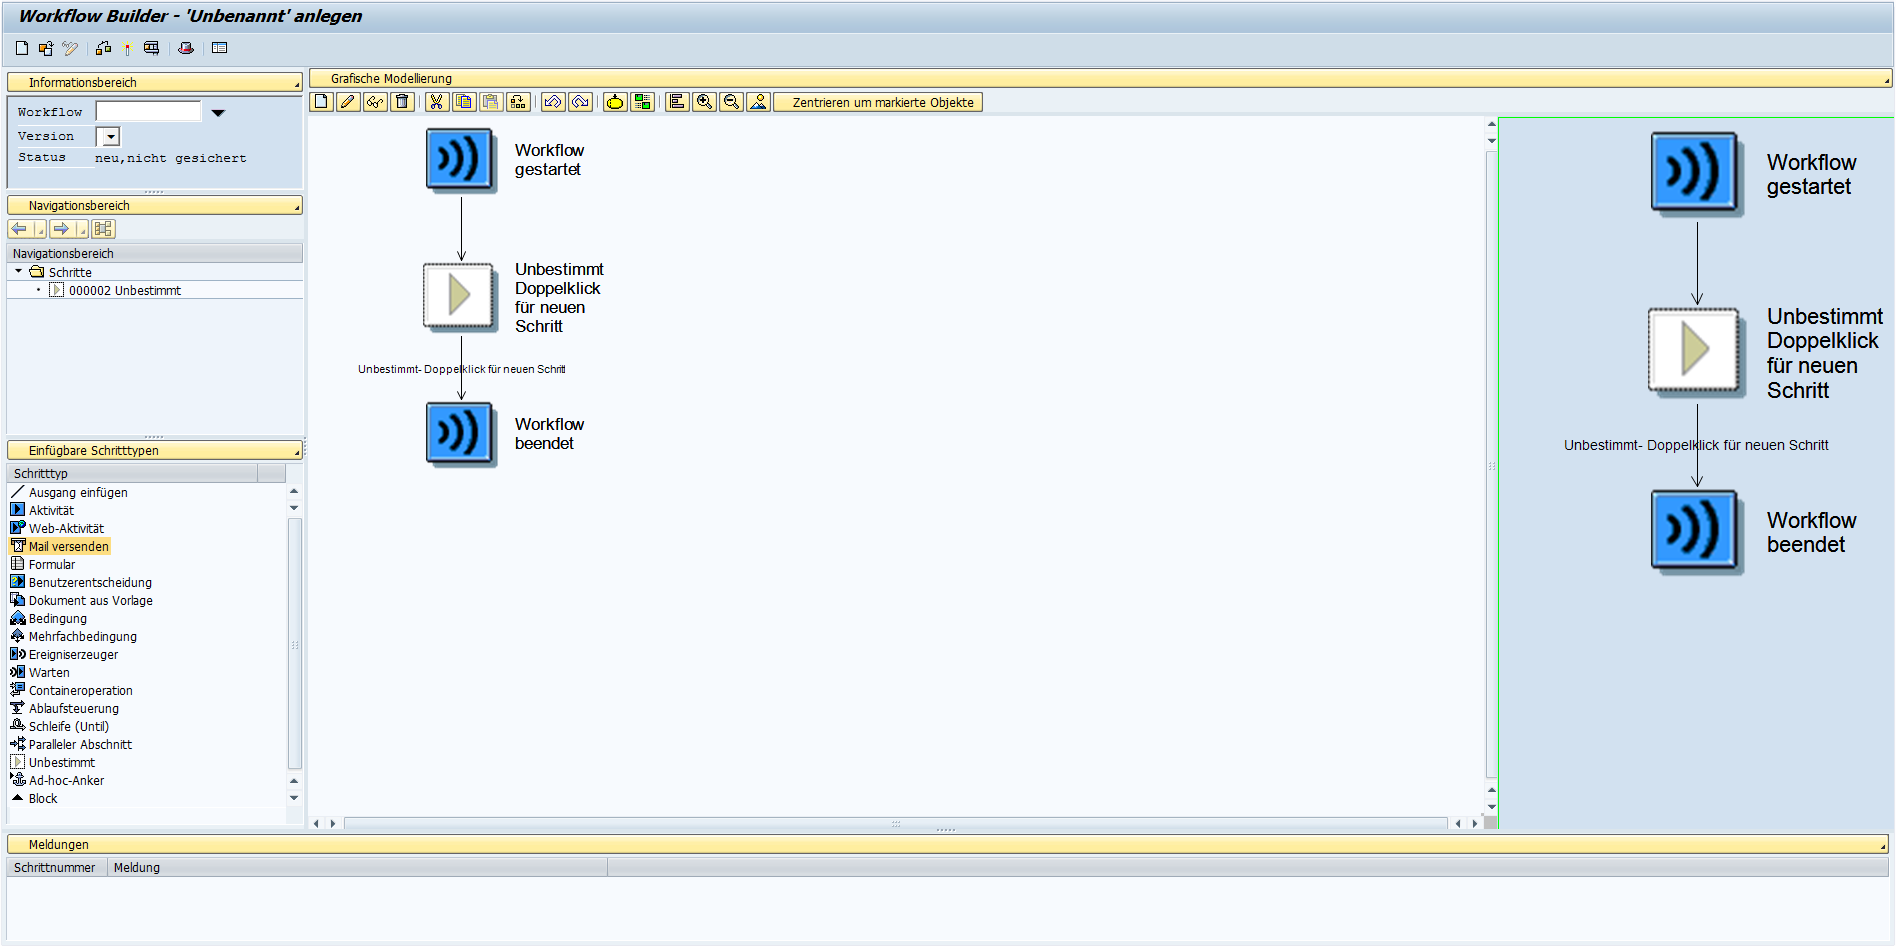
\includegraphics[width=1.0\textwidth]{grafiken/wf-builder_overview.png}
	\caption{Programmübersicht: Der SAP Workflow Builder}
	\vspace{-10pt}
	\label{abb:workflow-overview}
	\end{center}
\end{figure}

\subsubsection{Workflow}
\label{sec:win-overview-wf}
Dieser Bereich ist der wichtigste und größte. Hier wird der Bereich des modellierten Arbeitsablaufs, der gerade bearbeitet wird, groß dargestellt und es können neue Schritte eingefügt werden, vorhandene Schritte editiert und gelöscht werden. Ein Doppelklick auf einen Schritt bringt den Benutzer zur gespeicherten Definition des Elements, welche dort gepflegt werden kann.

\subsubsection{Übersicht}
\label{sec:win-overview-uebersicht}
Die grafische Übersicht bietet dem Bearbeiter stets einen Überblick des gesamten Workflows, wofür dieser bei großen Modellierungen stark verkleinert dargestellt werden muss. Zusätzlich signalisiert ein grüner rechteckiger Rahmen stets, welcher Teil des Gesamtbildes aktuell im großen Workflow Fenster bearbeitet wird. Durch Verschieben des Rahmens ist es möglich, direkt zu einem gewünschten Teil zu springen.

\subsubsection{Schritttypen}
\label{sec:win-overview-schrittypen}
Der untere linke Bereich des Programms hat standardmäßig den Titel "Einfügbare Schrittypen" und enthält eine Liste aller Schrittypen, die verwendet werden können. Von hier können diese mit der Maus per \gls{dragdrop} in den Prozess eingefügt werden. Beim Einfügen des Schrittes wird durch ein kleines Plus am Mauszeiger signalisiert, dass der entsprechende Schritt an dieser Stelle eingefügt werden kann.

\subsubsection{Informationsbereich}
\label{sec:win-overview-information}
Der Informationsbereich zeigt an, welcher Workflow aktuell geladen ist, dessen Status und Versionsnummer. Durch einen Klick auf die Auswahlliste neben "Version" kann eine andere Version des gespeicherten Prozesses geladen werden. Um einen neuen Prozess zu laden, kann entweder, wenn diese bekannt ist, die entsprechende Identifikationsnummer in das Textfeld neben "Workflow" eingegeben werden oder die Suchhilfe mittels des kleinen Pfeils daneben geöffnet werden. Letzteres öffnet das in Abbildung \ref{abb:workflow-search} gezeigte Fenster, in welchem die auf dem System vorhandenen Workflows nach Kategorien aufgegliedert angezeigt werden.

\begin{figure}[h]
	\begin{center}
	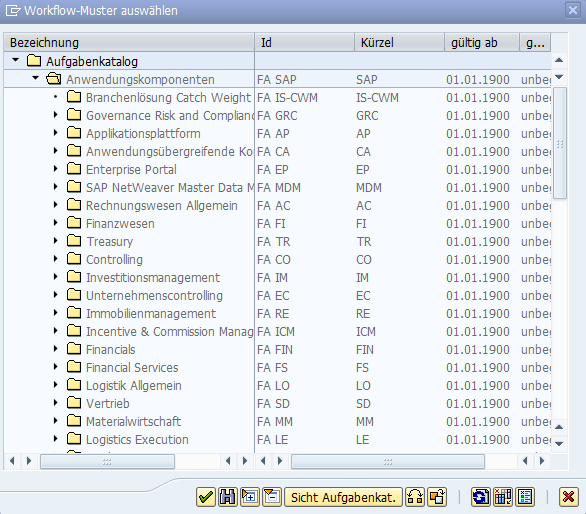
\includegraphics[width=300px]{grafiken/wf-builder_search.png}
	\caption{Die Suchhilfe des Workflow Builders}
	\vspace{-10pt}
	\label{abb:workflow-search}
	\end{center}
\end{figure}

\subsubsection{Navigationsbereich}
\label{sec:win-overview-information}
Der Navigationsbereich beinhaltet eine Liste aller im Prozess vorhandenen Schritte. Von hier aus ist es möglich, direkt zu der Definition eines gewünschten Schrittes zu springen. 

\subsubsection{Meldungen}
\label{sec:win-overview-meldungen}
In diesem Bereich werden Nachrichten zur Information des Benutzers angezeigt. Dies können allgemeine Benachrichtigungen, Ergebnisse der Syntaxprüfung und Suchergebnisse sein.

\subsubsection{Alternative Inhalte}
\label{sec:win-overview-alternative}
Zusätzlich zu den standardmäßig beim Programmstart und in Abbildung \ref{abb:workflow-overview} angezeigten Informationen kann die Ansicht \nameref{sec:win-overview-schrittypen} zu einer alternativen Ansicht geändert werden. Dies erfolgt, indem der Benutzer auf die Überschrift "Einfügbare Schritttypen" des Bereichs klickt. Aus dem nun geöffneten Menü (siehe \ref{abb:workflow-alternatives}) ist einer der Einträge auszuwählen. Die folgenden Ansichten stehen zur Verfügung:

\begin{figure}[h]
	\begin{center}
	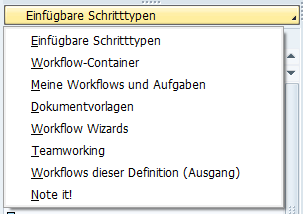
\includegraphics[width=150px]{grafiken/wf-builder_alternative-inhalte.png}
	\caption{Alternative Anzeigemöglichkeiten des Workflow Builders}
	\vspace{-10pt}
	\label{abb:workflow-alternatives}
	\end{center}
\end{figure}

\begin{enumerate}
	\item Der \textbf{Workflow Container} beinhaltet alle Elemente, wie Variablen und Benutzereingaben, welche während der Ausführung des Workflows benötigt werden. Neben den automatisch generierten Container Elementen können auch vom Benutzer definierte Elemente angelegt werden.
	\item Die Ansicht \textbf{Meine Workflows und Aufgaben} bietet einen Schnellzugriff auf alle Workflows, die in letzter Zeit bearbeitet wurden. Des weiteren kann eine eigene Liste an Aufgaben und Workflows angelegt werden.
	\item \textbf{Dokumentvorlagen} sind Dokumente externer Programme (Excel-Tabellen, Word-Dateien oder beliebige andere), welche im Schritt "Dokument aus Vorlage" eingebunden werden können. 
	\item \textbf{Workflow Wizards} bieten dem Benutzer die Möglichkeit, häufig genutzte Prozessteile mit Hilfe eines von \gls{sap} bereitgestellten \gls{wizard}s einzufügen.
	\item In der Ansicht \textbf{Teamworking} kann nach Schritten gesucht werden, welche von einer bestimmten Person als letztes bearbeitet wurden.
	\item Der Punkt \textbf{Workflows dieser Definition (Ausgang)} zeigt alle zur Zeit auf dem System ausgeführten Instanzen dieser Workflow Version.
	\item Der letzte Punkt, \textbf{Note it!} bietet dem Benutzer die Möglichkeit, sich Notizen zu seiner aktuellen Arbeit zu erstellen.
\end{enumerate}



\subsection{Funktionen des Builders}
\label{sec:builder-funktionen}
% MARCO
% welche Funktionalitäten hat der Builder...
Im Folgenden sollen nun zuerst die wichtigsten Funktionen des \gls{sap} Workflow Builders erklärt werden. Danach folgt im Kapitel \nameref{sec:builder-elemente} eine breiter gefächerte tabellarische Übersicht. Dort sind auch die Symbole der Schrittypen mit aufgeführt. 

Beim ersten Start des Programms wird dem Benutzer statt einer leeren Arbeitsfläche der minimale Aufbau eines Workflows im \gls{sap}-System angezeigt. (Siehe hierzu Abbildung \ref{abb:workflow-easy}) Dieser besteht aus dem Startereignis "`Workflow gestartet"' und dem Endereignis "`Workflow beendet"'. Dazwischen können beliebige Schritte an Stelle des unbekannten Schrittes (gekennzeichnet durch einen Pfeil auf weißem Hintergrund) eingefügt werden.

\begin{figure}[h]
	\begin{center}
	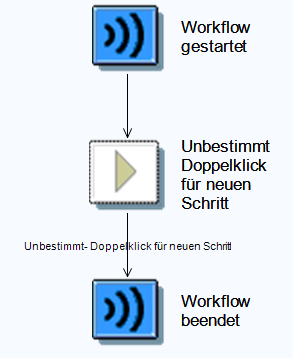
\includegraphics[width=150px]{grafiken/wf-builder_new-wf.png}
	\caption{Der initiale Workflow des Builders}
	\vspace{-10pt}
	\label{abb:workflow-easy}
	\end{center}
\end{figure}

\subsubsection{Aktivität}
Der wichtigste Schritttyp ist die Aktivität, welche verschiedene Aufgaben erfüllen kann. Der Benutzer kann entweder einen \gls{abap} \gls{objekttyp} und eine zugehörige Methode oder eine im System vorhandene und schon definierte Aufgabe auswählen. Die entsprechende Aktivität wird dann vom System automatisch gestartet, wenn die Stelle im laufenden Workflow erreicht wird \cite{SAPHelpWf}.

\subsubsection{Web-Aktivität}
Mit Hilfe dieses Schrittes wird aus dem internen Workflow heraus ein XML-Dokument an eine URL gesendet. Der Empfänger kann beispielsweise ein anderes System sein, welches daraufhin einen eigenen Workflow startet. Alle \gls{sap}-Systeme stellen einen Service zur Verfügung, welcher in diesem Fall automatisch einen weiteren Workflow starten kann \cite{SAPHelpWf}.

\subsubsection{Mail versenden}
Dieser Schritt versendet eine Nachricht innerhalb des \gls{sap}-Systems. Der Empfänger (es sind mehrere Empfänger möglich) kann diese im internen Postfach abrufen. Der Text der Mail wird bei der Definition des Schrittes festgelegt, wobei Variablen verwendet werden können, welche zur Laufzeit mit den entsprechenden Werten gefüllt werden \cite{SAPHelpWf}.

\subsubsection{Formular}
Ein Formular kann innerhalb des Workflows zur Anzeige von Daten oder deren Bearbeitung durch den Endnutzer verwendet werden. Nachdem bei der Definition des Schrittes die zu bearbeitenden Daten angegeben wurden, erzeugt das Workflow-System automatisch das zugehörige Formular, welches noch bearbeitet werden kann \cite{SAPHelpWf}. 

\subsubsection{Benutzerentscheidung}
Eine Benutzerentscheidung kann mit einem Text versehen werden, welcher dem Endnutzer erklärt, welche Entscheidung er treffen muss. Der Workflow kann so konfiguriert werden, dass er, je nachdem welche der vorgegebenen Antwortmöglichkeiten ausgewählt wurde, einen anderen Pfad wählt \cite{SAPHelpWf}.

\subsubsection{Bedingungen}
Die Schritte Bedingung und Mehrfachbedingung bestimmen, ähnlich der Benutzerentscheidung, den weiteren Ablauf des Workflows. Der Unterschied besteht darin, dass das System die Entscheidung eigenständig nach vorgegebenen Bedingungen fällt und der Benutzer keinen Einfluss darauf hat \cite{SAPHelpWf}.

\subsubsection{Schleifen}
Die WHILE- und UNTIL-Schleifen können eingesetzt werden, wenn ein bestimmter Teil des Workflows ausgeführt werden soll, während eine bestimmte Bedingung wahr ist oder so lange, bis sie eintritt. Schleifen können sämtliche Schrittypen (auch weitere Schleifen) enthalten und sorgen dafür, dass ein Workflow übersichtlich bleibt \cite{SAPHelpWf}.

\subsection{Schritttypen}
\label{sec:builder-elemente}
% MARCO, STEFFEN
% tabelle mit elementen..
% was ist wofür gedacht
	\begin{longtable}{|c|p{2.2cm}|p{10.8cm}|}
		\hline
		\textbf{Symbol} & \textbf{Schritttyp} & \textbf{Beschreibung}\\
		\hline
		\includegraphicstotab[width=0.8cm]{grafiken/aktivitaet.png}
		& 
		Aktivität & Ausführen einer ABAP-Methode oder einer vordefinierten Aufgabe \\ 
		\hline \includegraphicstotab[width=0.8cm]{grafiken/web-aktivitaet.png} 
		& 
		Web-Aktivität & \gls{xml}-Dokument an eine URL senden, z.B. um Workflows in Fremdsystemen zu starten\\ 
		\hline 
		\includegraphicstotab[width=0.8cm]{grafiken/mail-versenden.png} 
		& 
		Mail-Versendung & Nachricht an Endnutzer versenden\\ 
		\hline 
		\includegraphicstotab[width=0.8cm]{grafiken/formular.png}
		& 
		Formular-schritt & Anzeige von Daten und Möglichkeit zum Bearbeiten dieser durch Endnutzer\\ 
		\hline 
		\includegraphicstotab[width=0.8cm]{grafiken/benutzerentscheidung.png}
		& 
		Benutzer-entscheidung & Beantworten einer Frage bzw. Treffen einer Entscheidung durch den Benutzer zur Beeinflussung des Workflows\\ 
		\hline 
		\includegraphicstotab[width=0.8cm]{grafiken/dokument-aus-vorlage.png}
		& 
		Dokument aus Vorlage & Anzeigen oder Bearbeiten von Dokumenten, die mit externen Anwendungen erstellt wurden mit Hilfe eines auf dem Rechner installierten Programms\\ 
		\hline 
		\includegraphicstotab[width=0.8cm]{grafiken/bedingung.png}
		& 
		Bedingung & Bedingte, selbstständige Entscheidung für einen Pfad aus zwei Möglichkeiten durch das System\\ 
		\hline 
		\includegraphicstotab[width=0.8cm]{grafiken/mehrfachbedingung.png}
		& 
		Mehrfach-bedingung & Bedingte, selbstständige Entscheidung für einen Pfad aus mehreren Möglichkeiten durch das System\\ 
		\hline 
		\includegraphicstotab[width=0.8cm]{grafiken/ereigniserzeuger.png}
		& 
		Ereignis-erzeuger & Auslösen eines Ereignisses, auf welches ein Warteschritt wartet\\ 
		\hline 
		\includegraphicstotab[width=0.8cm]{grafiken/warten.png}
		& 
		Warteschritt & Warten, bis ein durch einen Ereigniserzeuger generiertes Ereignis eintritt\\ 
		\hline 
		\includegraphicstotab[width=0.8cm]{grafiken/containeroperationen.png}
		& 
		Container-operationen & Verändern von Elementen des Workflow-Containers (Umgebung des aktiven Workflows mit Variablen und Benutzerentscheidungen)\\ 
		\hline 
		\includegraphicstotab[width=0.8cm]{grafiken/ablaufsteuerung.png}
		& 
		Ablauf-steuerung & Eingriff in den Ablauf des aktuellen Workflows - Abbruch oder Beenden einzelner Schritte oder des gesamten Workflows\\ 
		\hline 
		\includegraphicstotab[width=0.8cm]{grafiken/schleife.png}
		& 
		Schleifen & Mehrfache Ausführung eines Blocks von Schritten unter einer bestimmten Bedingung\\ 
		\hline 
		\includegraphicstotab[width=0.8cm]{grafiken/paralleler-abschnitt.png}
		& 
		Paralleler Abschnitt & Aufsplitten des Workflows in zwei parallel laufende Pfade\\ 
		\hline 
		\includegraphicstotab[width=0.8cm]{grafiken/ad-hoc-anker.png}
		& 
		Ad-hoc-Anker & Möglichkeit, einen anderen Workflow des Systems zu hinterlegen, der vom berechtigten Benutzer ausgeführt werden kann\\ 
		\hline 
		\includegraphicstotab[width=0.8cm]{grafiken/block.png}
		& 
		Block & Zusammenfassen mehrerer Schritte zu einem Block mit eigenen Variablen\\ 
		\hline 
		\includegraphicstotab[width=0.8cm]{grafiken/lokaler-workflow.png}
		& 
		Lokaler Workflow & Einfügen eines Sub-Workflows, welcher vollen Zugriff auf die Daten des aktuellen Workflows hat\\ 
		\hline
	% Beschriftung festlegen:
	\caption{Symbolerklärung des \gls{sap} Workflow Builders}
	% ein Label definieren, mit dessen Hilfe man (an beliebiger Stelle im Dokument) Bezug nehmen kann:
	\label{tab:builderelemente}		
	\end{longtable} 



%%%%%%%%%%%%%%%%%%%%%
%% KAPITEL HandsOn %%
%%%%%%%%%%%%%%%%%%%%%
%% MARCO
%%%%%%%%%%%%%%%%%%%%%
\section{Hands On}

\subsection{Erster Beispielworkflow}
\label{sec:builder-1-bsp}
% kleiner sinnloser workflow (schleife,...) => aus dem Video Tutorial

\subsection{Zweiter Beispielworkflow}
\label{sec:builder-2-bsp}
% demo workflow aus den vorlagen nehmen (abwesenheitsbestätigung)

\subsubsection{Vorstellung des Workflows}
\label{sec:builder-2-bsp-vorstellung}
% wofür ist der workflow gut, was soll er tun (aus anwendersicht)

\subsubsection{Umsetzung des Workflows}
\label{sec:builder-2-bsp-umsetzung}
% technische sicht, "`klickbares"' howto

%%%%%%%%%%%%%%%%%%%%%%%%%%
%% KAPITEL Fremdsysteme %%
%%%%%%%%%%%%%%%%%%%%%%%%%%
%% JONAS 
%%%%%%%%%%%%%%%%%%%%%%%%%%
\section{Schnittstellen}

\subsection{SAP Fremdsysteme}
\label{sec:export-sap}

\gls{sap} Systeme liefern Workflows, die die Aufgaben des Systems in computerverständlicher Form darstellen. \gls{erp}, \gls{crm} und \gls{srm} sind Beispiele für Systeme, die eingebaute, vordefinierte Workflows bereitstellen. Mit diesen Geschäftsprozessen können \gls{zb} der Verlauf einer Bestellung oder dem Verwalten von Lieferketten dargestellt werden.

Die Workflows sind anpassbar, um den Bedürfnissen der Firma gerecht zu werden. Vor dem Einsatz der \gls{sap}-Lösung kann der Kunde die gewünschten Geschäftsprozesse genau auf sein Unternehmen zuschneiden. 

Es können mit dem Workflowbuilder eigene Geschäftsprozesse entwickelt werden. Die aus bestehenden Workflow-Management System importiert werden können. So kann der Kunde relativ einfach sein vorhandenes Setup wiederverwenden.

Da die Einzelnen Aktivitäten der Workflows aus ABAP-Klassen bestehen können Geschäftsprozesse im Workflowbuilder natürlich über Modulgrenzen hinweg auf Daten anderer Systeme zugreifen. So können \gls{zb} Daten aus einem \gls{crm}-System in einem \gls{erp} zur Analyse, Auswertung und Bearbeitung von Daten hinzugezogen werden.

\subsection{XML}
\label{sec:export-xml}
% was ist dieses Format
% in welche Programme kann man es importieren?

\gls{xml} ist die Abkürzung für E\textbf{x}tensible \textbf{M}arkup \textbf{L}anguage und bezeichnet eine Auszeichnungssprache. Mit dieser können hierarchisch strukturierte Daten in Textform dargestellt werden. \gls{xml} besteht aus Elementen, deren Name, bis auf ein paar Ausnahmen, frei gewählt werden darf. Elemente haben einen Anfangs- ($\langle$elementName$\rangle$) und einen Endtag ($\langle$/elementName$\rangle$). Zwischen den Tags können weiter Elemente, Text und Knoten stehen. Diese sind dem Element dann untergeordnet.

Das World Wide Web Consortium, kurz \gls{w3c}, hat \gls{xml} als eine Metasprache definiert, auf deren Basis anwendungsspezifische Auszeichnungssprachen entwickelt werden können. Diese werden beschrieben durch ein Schema, welches festlegt, welche Elemente verwendet werden dürfen und welches Verhalten diese aufweisen \cite{XML}. So ist \gls{zb} auch XHTML definiert.

\subsection{BPMN}
\label{sec:export-bpmn-bpml}
% was ist dieses Format
% in welche Programme kann man es importieren?

\textbf{B}usiness \textbf{P}rocess \textbf{M}odel and \textbf{N}otation (\gls{bpmn}) ist eine grafische Spezifikationssprache, welche Symbole bereitstellt mit deren Hilfe Geschäftsprozesse und Arbeitsabläufe dargestellt werden können.\cite{BPMN} \gls{bpmn} wurde 2005 von der \gls{omg}, auch zuständig für \gls{zb} \gls{uml}, übernommen und gewann ab dann an Bedeutung in der Informatik. Außerdem wurde sie 2013 zum internationalen Standard (ISO/IEC 19510:2013) erhoben \cite{OMG}.

Da sich \gls{bpmn} rein auf die Darstellung von Workflows bezieht wurden mehrere, von \gls{xml} abgeleitete, Auszeichnungssprachen entwickelt, um Business Process Models auch als, für einen Computer verständliche, Daten aufschreiben zu können. Dazu zählen \gls{zb} \gls{bpel}, \gls{xpdl} oder \gls{bpml} \cite{BPMN}.

\subsubsection{BPML}

Die \textbf{B}usiness \textbf{P}rocess \textbf{M}odeling \textbf{L}anguage (\gls{bpml}) wird von \gls{sap} im Workflowbuilder (\ref{chap:builder}) verwendet um Geschäftsprozesse zu exportieren. Da \gls{bpml} auch unter dem Dach der \gls{omg} steht wird sie auch in anderen Workflow Management Systemen, wie \gls{zb} jBPM, Camunda BMP oder ARIS, verwendet. Dadurch lassen sich \gls{sap}-interne Geschäftsprozesse auch extern einbetten \cite{BPML}.